\begin{frame}{Governance structure of Tokyo government}
    \begin{itemize}
        \item Tokyo government was a public institution managing the central areas of Tokyo\footnote{Later (1945-) expanded to the entire Tokyo prefecture.}.

        \item The government consisted of approximately 40,000 employees to support the 7,000,000 citizens in Tokyo.

        \item The government provided a wide range of public goods (Transportation, Health service, Port control, Education, etc)\footnote{Not sure about procurement practices.}
             

\
        
        \item Staff was allocated to 12 departments. 
        \begin{enumerate}
            \item Each department was assigned a type of public good to supervise and provide.
            \item Departments were split into offices. 
            \item Offices were further divided into units. A unit consists of approximately 10-15 workers.
        \end{enumerate} 
        \

        \item Many offices/units were added/removed each year (in 1935-1937 approx 15\% of offices were removed).
    \end{itemize}

    
    
\end{frame}

\begin{frame}{Example of Multidivisional Structure}
    \begin{figure}
        \centering
        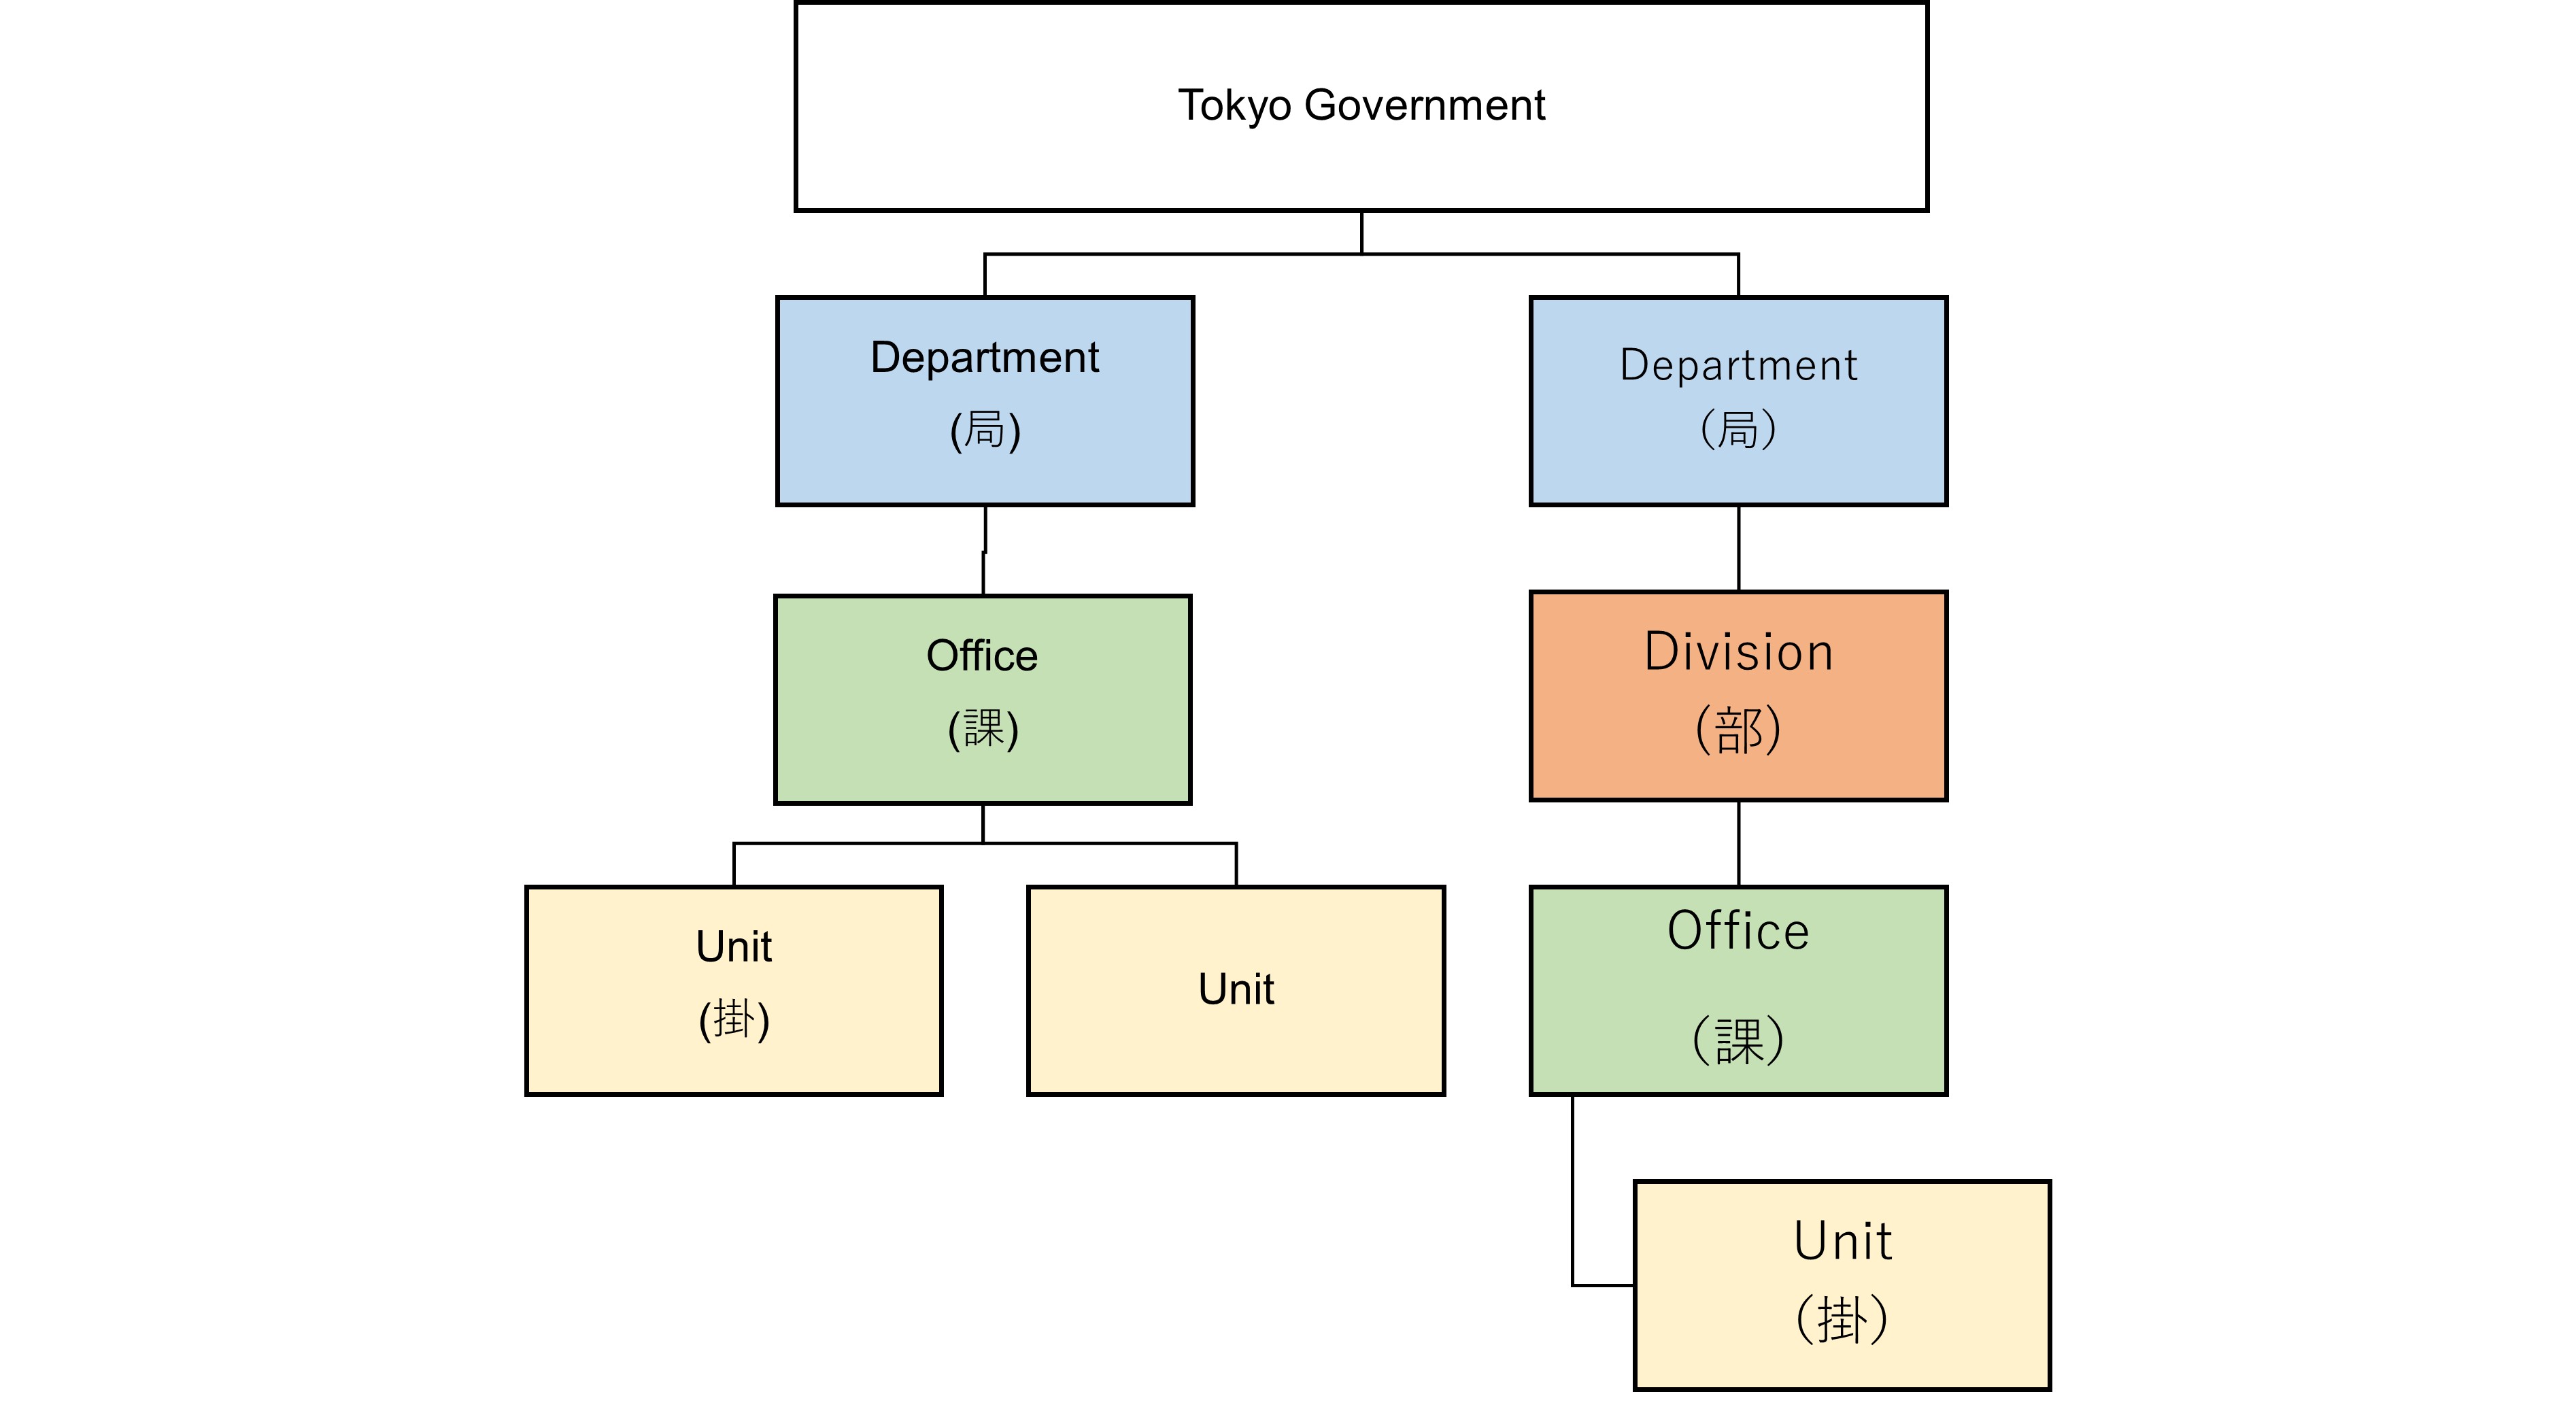
\includegraphics[height=0.8\textheight]{Institutional Background/HierarchyChart.png}
        \label{fig:enter-label}
    \end{figure}
\end{frame}

\begin{frame}{Multidivisional Structure}
    \begin{figure}
        \centering
        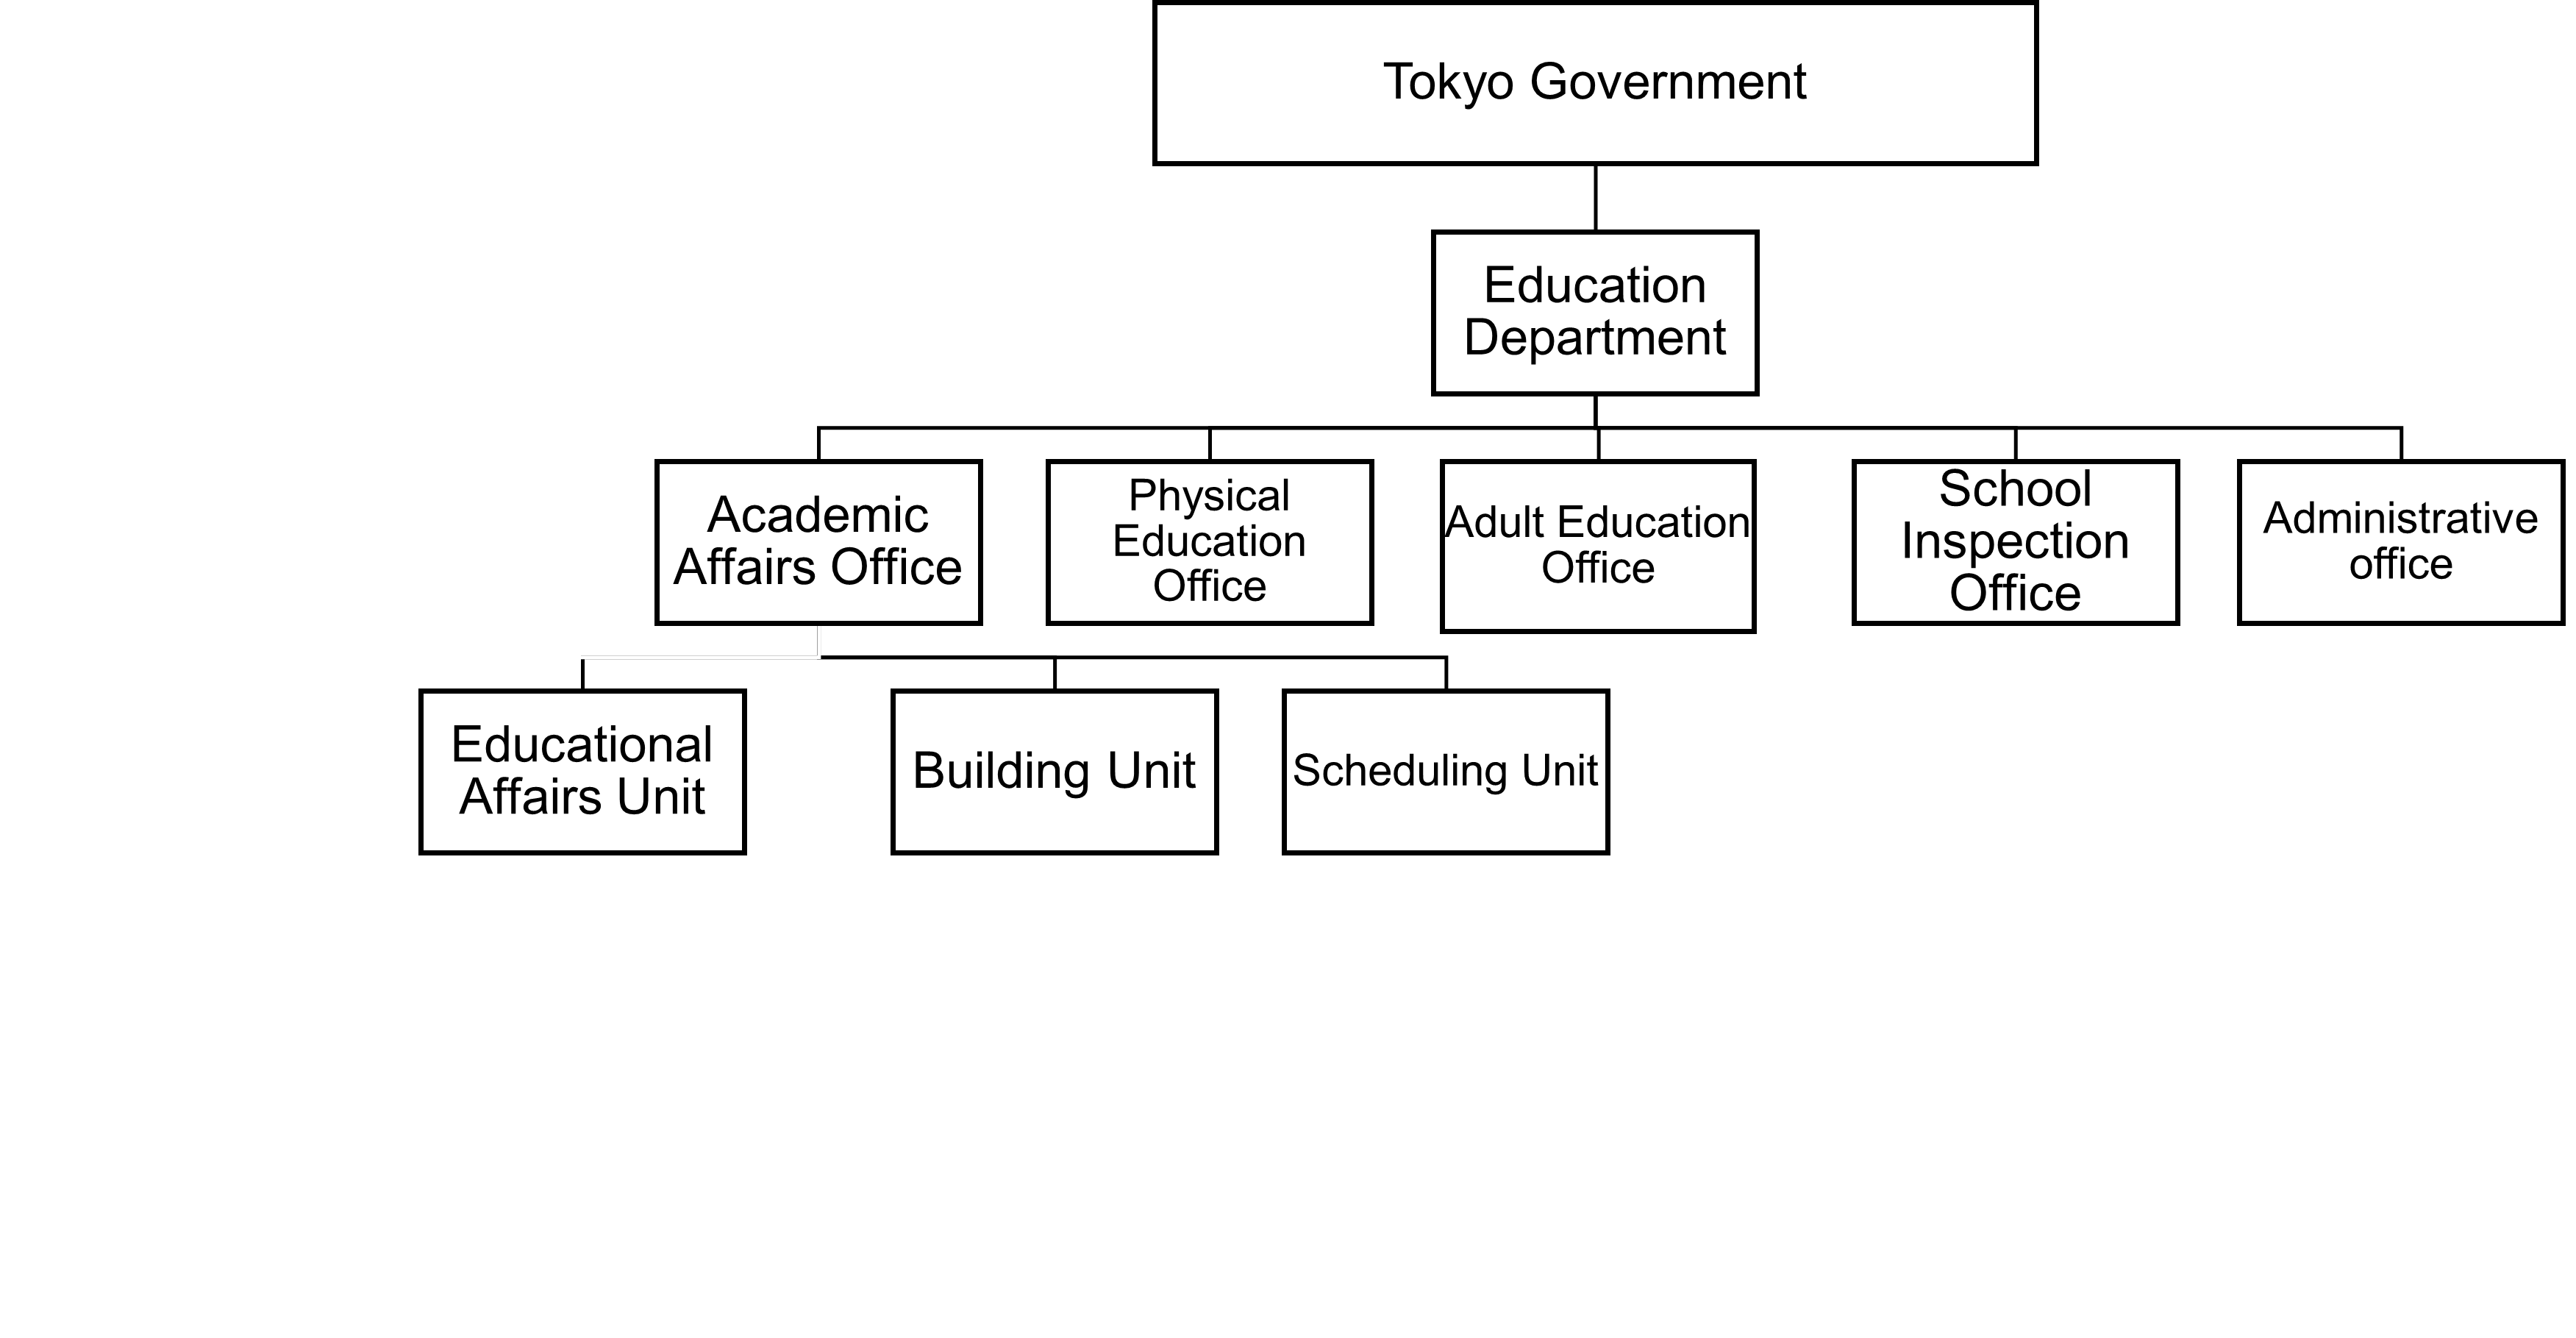
\includegraphics[width=1.1\textwidth]{Institutional Background/DeptEducation.png}
        \label{fig:enter-label}
    \end{figure}
\end{frame}

\begin{frame}{Attributes of offices}
     \begin{figure}
         \centering
         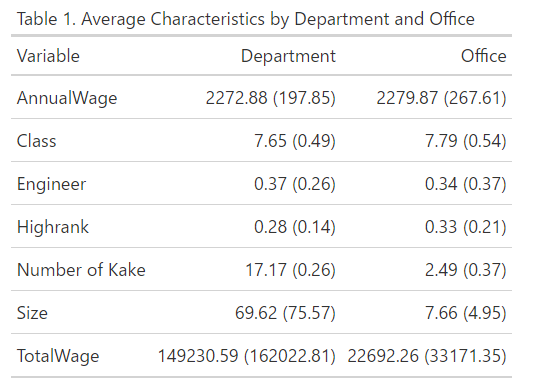
\includegraphics[width=\textwidth]{Institutional Background/OfficeAttributes.png}
         \label{fig:enter-label}
     \end{figure}
\end{frame}

%\begin{frame}{Transition of Offices/Departments}
%     \begin{figure}
%         \centering
%         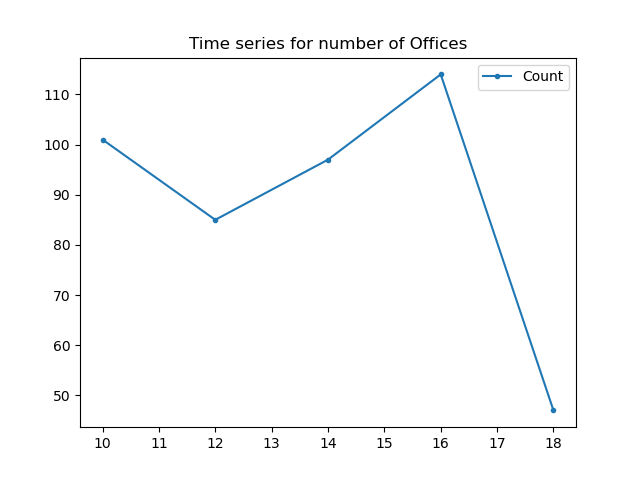
\includegraphics[width=\textwidth]{Institutional Background/OfficeCount.png}
%         \label{fig:enter-label}
%     \end{figure}
%\end{frame}

\begin{frame}{Entry of Female workers}
    \begin{itemize}
        \item A unit would usually consist of a manager, clerks or engineers, and assistants.

        \

        \item During the war period, female workers were mainly hired as assistants to support unit leaders with their tasks.    
        \item Women were hired in offices with lower rate of engineers.
        
        \

        \item Female workers' continuation/promotion depended on the approval of the unit manager.

        $\Rightarrow$ Male incumbent's relation with female entrants:
        \begin{enumerate}
            \item Unit Manager: Direct subordinate.
            \item Clerk, engineers, and others: Co-workers.
        \end{enumerate}

        \


    \end{itemize}
\end{frame}

\begin{frame}{Assignment of workers to office/units}
\begin{itemize}
    \item Employees were all assigned an occupation (Engineer, Manager, Clerk, Assistant, etc) and a class indicating their profession and experience.
        
    \item Occupations were assigned upon entry to the government, although switching across occupations occasionally happened.

    \

    \item Non-assistant employees were hired and assigned to positions based on exams and internal assessments.

    \item Civil Servants were further categorized into upper/lower class.

    Upper Class: Managers.
    
    Lower Class: Clerks, Engineers, etc.

    \

    \item Department heads were often recruited from the central government. 
\end{itemize}
\end{frame}

\begin{frame}{Wage Chart}
    \begin{figure}
        \centering
        
\includegraphics[width=\textwidth]{Institutional Background/WageChart.png}
        \label{fig:enter-label}
    \end{figure}
\end{frame}



\begin{frame}{Public Servants' attributes}
    \begin{figure}
        \centering
        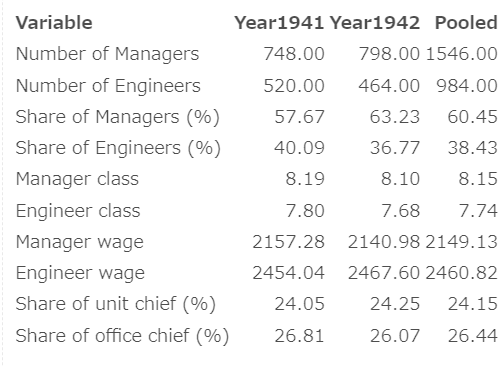
\includegraphics[width=\textwidth]{Institutional Background/UpperWorkerAttributes.png}
        \label{fig:enter-label}
    \end{figure}
\end{frame}


%\begin{frame}
%    \begin{figure}
%        \centering
%        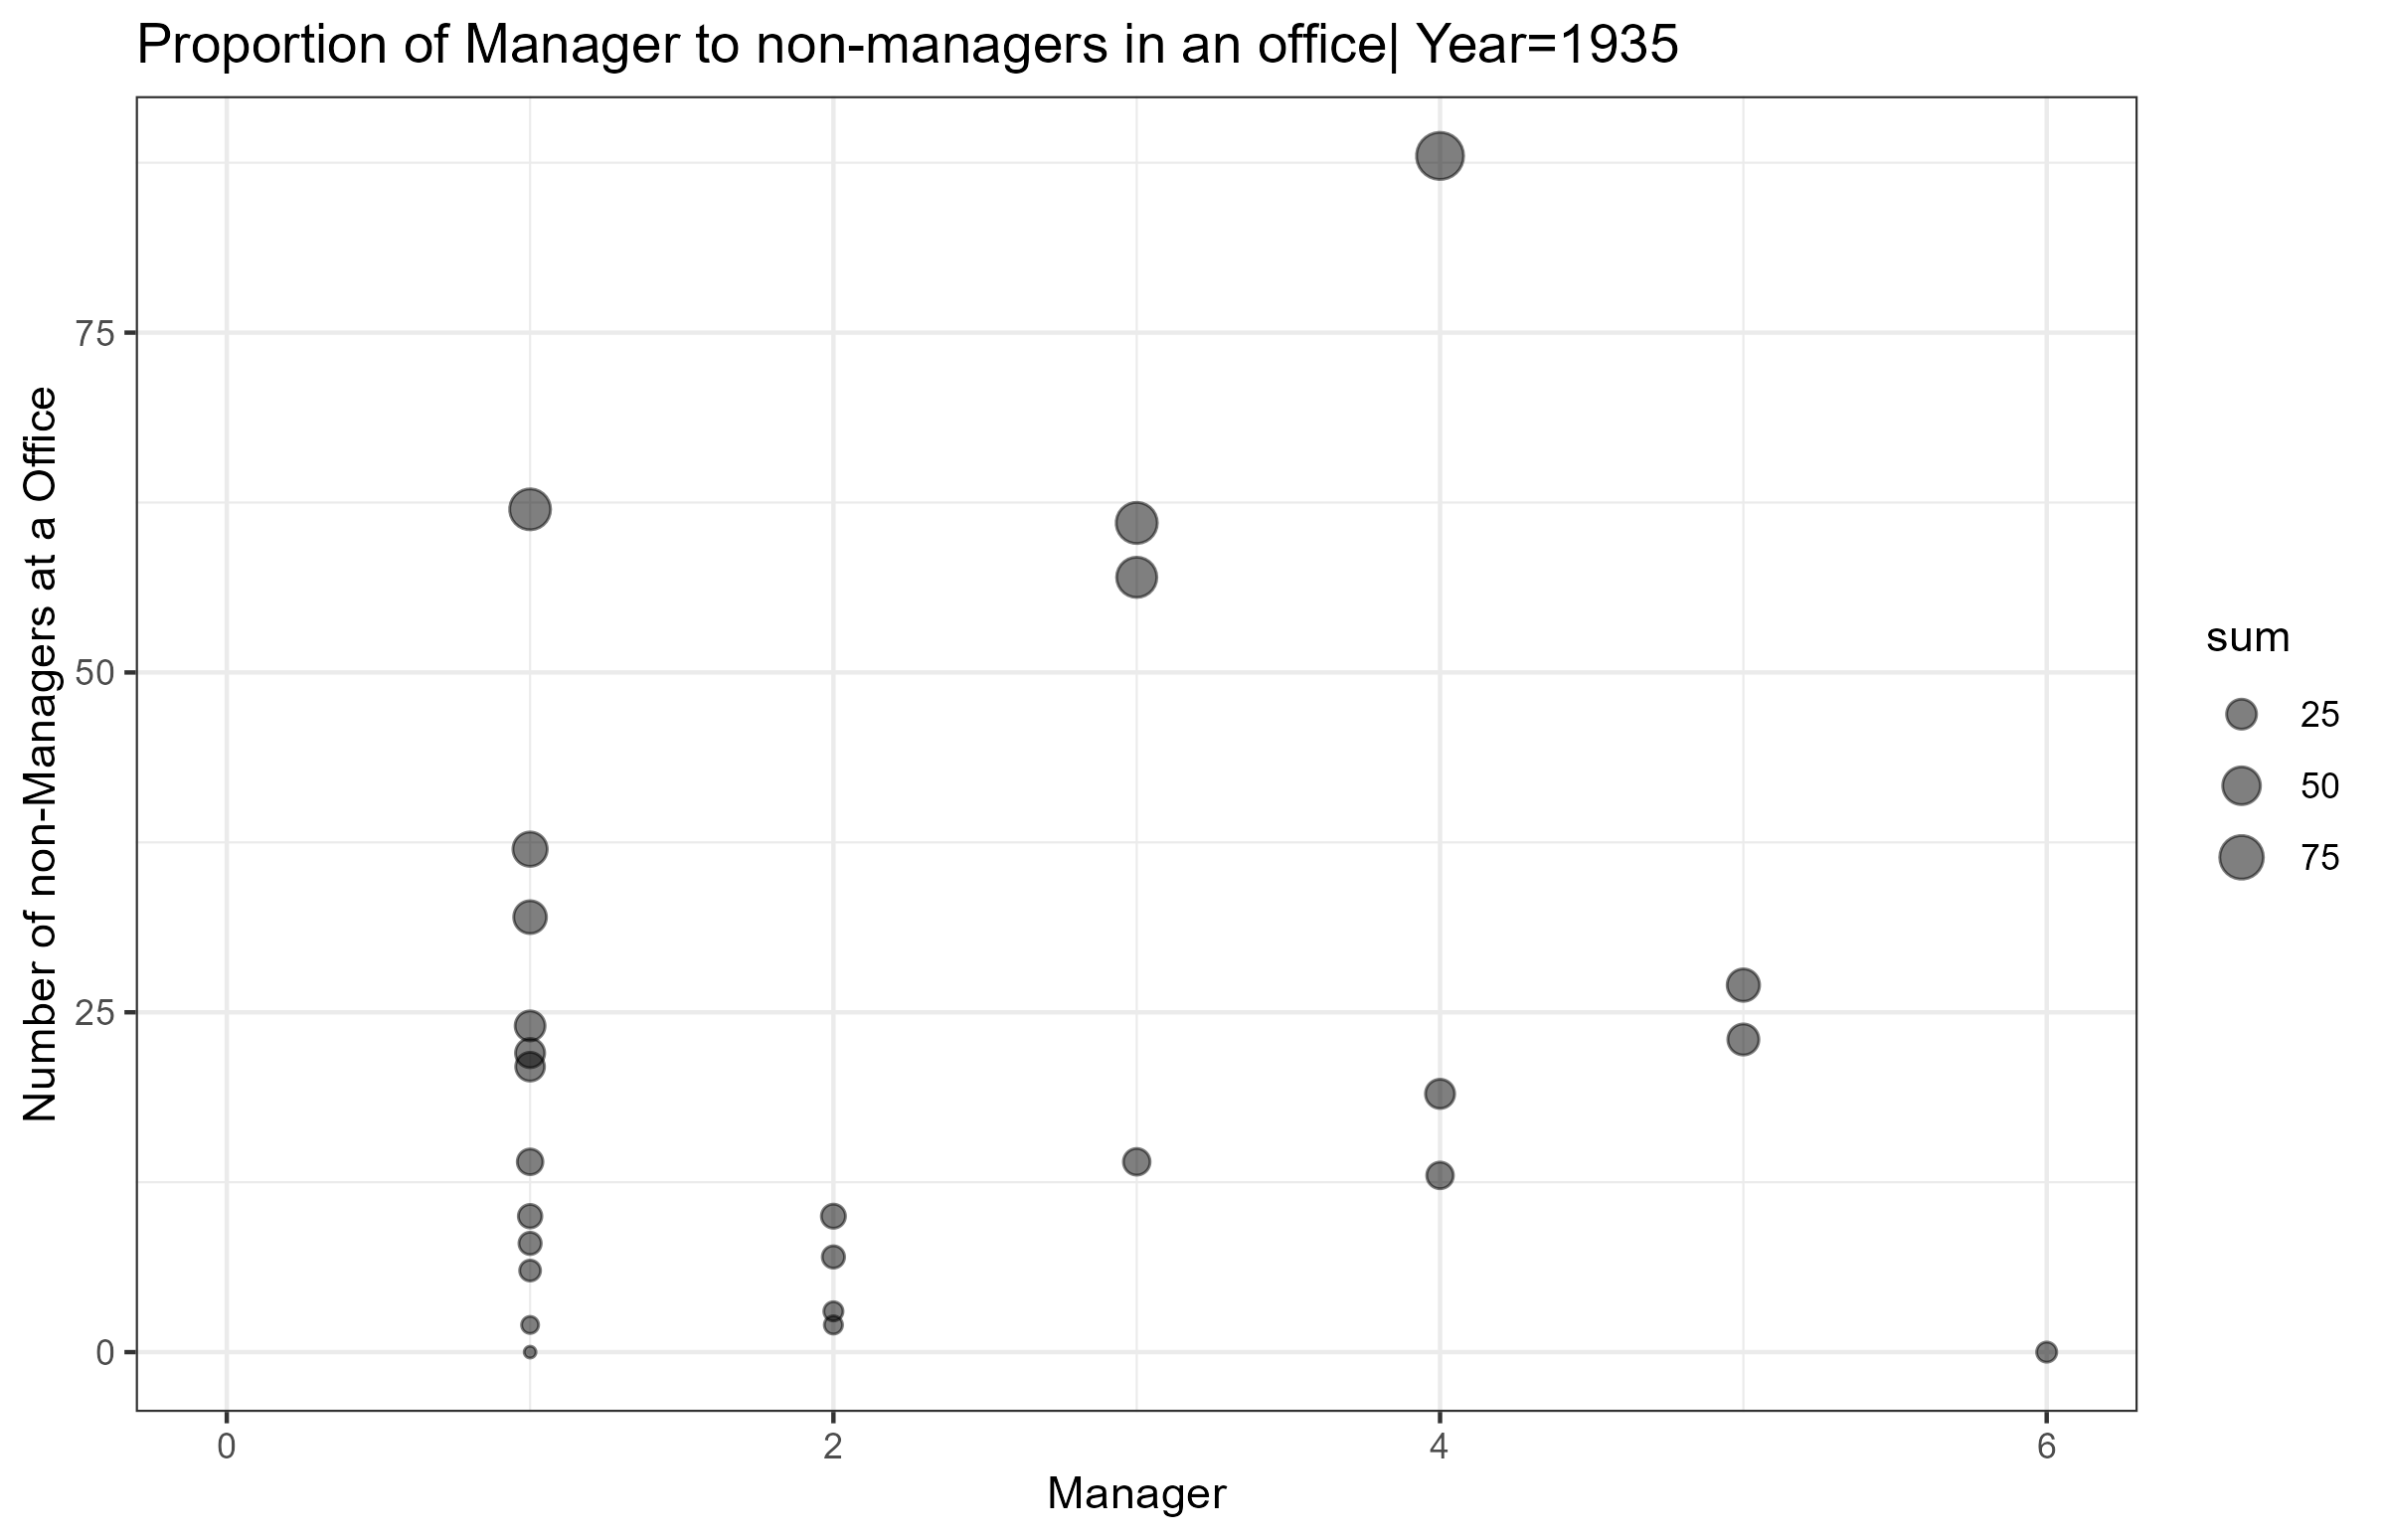
\includegraphics[width=\textwidth]{Institutional Background/Scatter_Agg.png}
%        \label{fig:my_label}
%    \end{figure}
%\end{frame}

%\begin{frame}
%    \begin{figure}
%        \centering
%        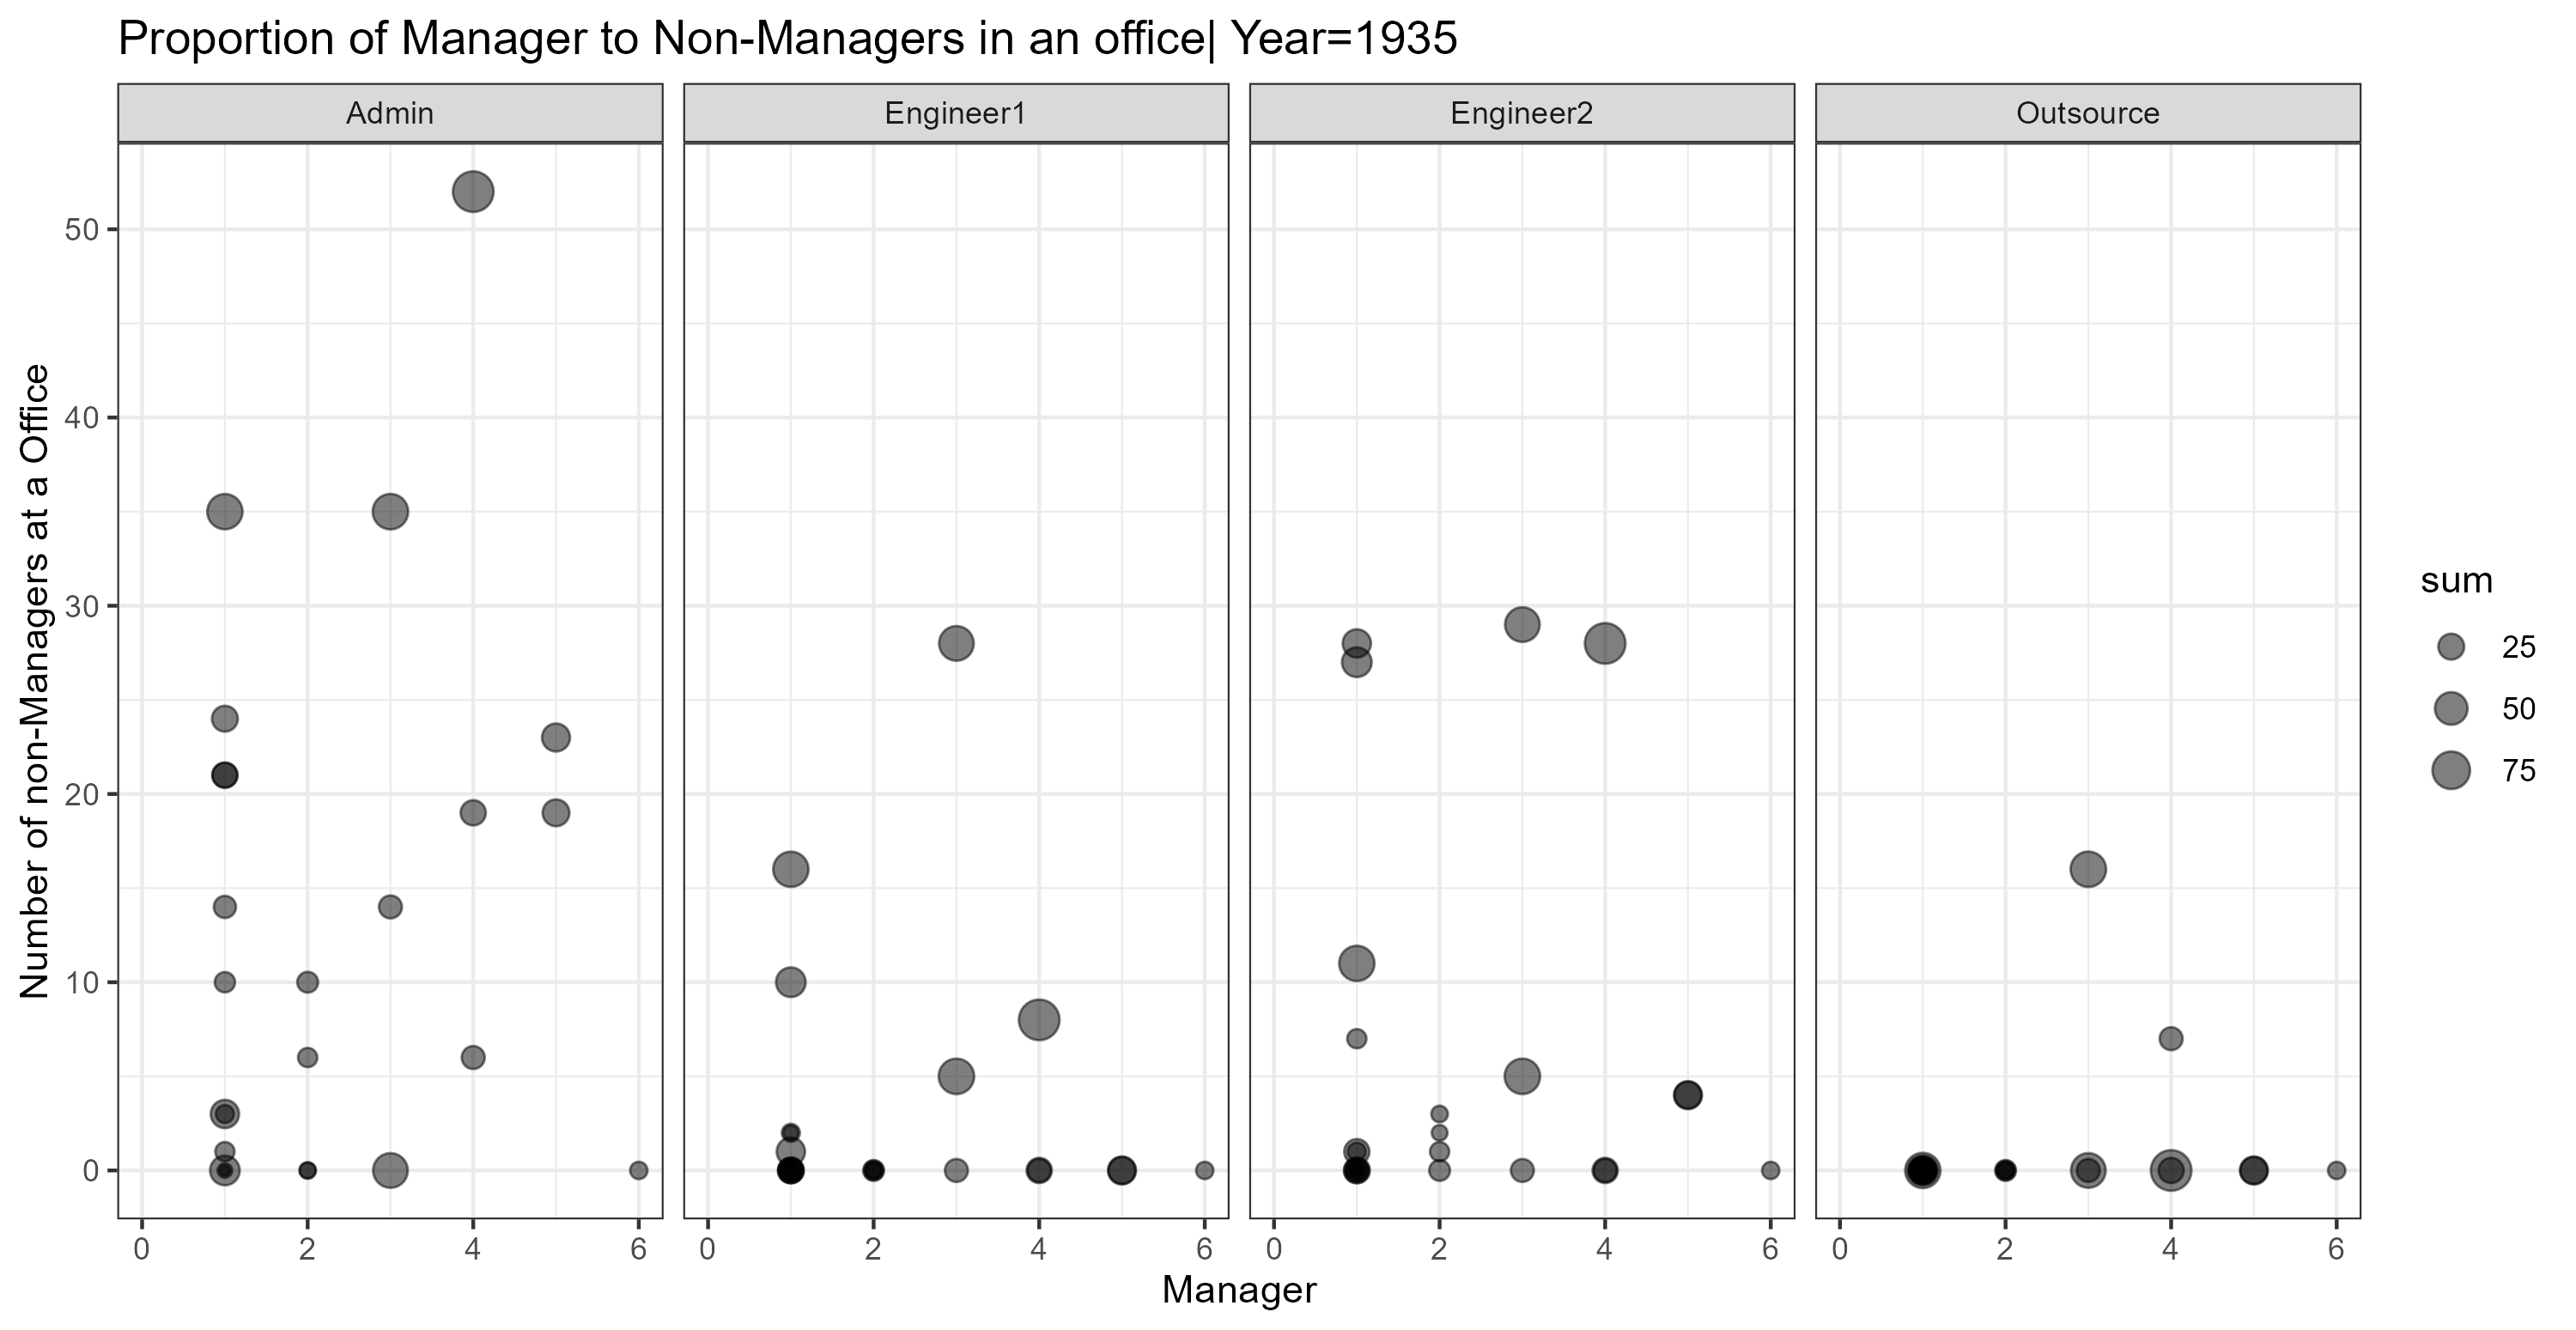
\includegraphics[width=\textwidth]{Institutional Background/Scatter_Occupation.png}
%        \label{fig:my_label}
%    \end{figure}
%\end{frame}




%\begin{frame}{Female labor force}
%    \begin{figure}
%        \centering
%        \includegraphics[width=\textwidth]{Institutional Background/Female_distribution.png}
%        \caption{Frequency plot of number of female workers in a city councils}
%        \label{fig:my_label}
%    \end{figure}
%\end{frame}

